% MATERIAIS E MÉTODOS------------------------------------------------------------------

\chapter{MATERIAIS E MÉTODOS}
\label{chap:metodologia}
Neste capítulo serão descritos os materiais e métodos utilizados no desenvolvimento da aplicação KeeMe, bem como as tecnologias que foram empregadas em sua construção. A Seção \ref{sec:desenvolvimento} descreve o processo de desenvolvimento utilizado na criação da ferramenta, discorrendo sobre as etapas do desenvolvimento e o que foi feito em cada uma delas. Já a Seção \ref{sec:gerenciamentoDaAplicacao} abordará a metologia que foi utilizada para fazer o gerenciamento do projeto como um todo. Na Seção \ref{sec:modelagem} será descrita a modelagem da aplicação, e aborda a UML, linguagem visual para modelagem e quais de seus recursos foram usados no desenvolvimento dessa aplicação. A Seção \ref{sec:prototipacao} discorrerá sobre a etapa de prototipação da interface do sistema e da estratégia utilizada para tanto. E por último, a Seção \ref{sec:tecnologias} discorrerá sobre tecnologias que foram utilizadas na criação da ferramenta.

\section{Processo de Desenvolvimento}
\label{sec:desenvolvimento}

\begin{figure}[H]
    \centering
    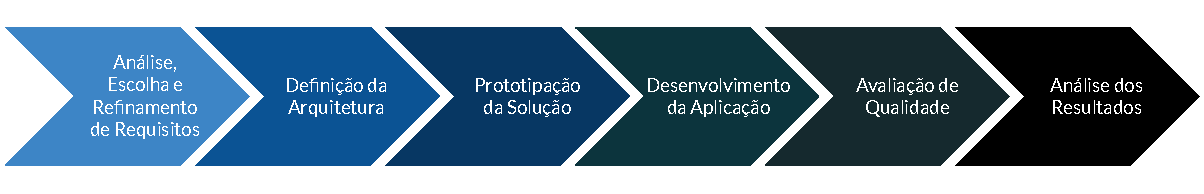
\includegraphics[width=\textwidth]{dados/figuras/Metodologia/grafico_evolutivo.pdf}
    \caption{Processo de desenvolvimento}
    \label{fig:processoDeDesenvolvimento}
\end{figure}

Durante o decorrer deste trabalho foi utilizado um Modelo Incremental para o seu desenvolvimento, descrito por \cite{dias2019__modelo_incremental} como uma evolução do Modelo Cascata, no qual ao invés de se especificar e desenvolver tudo de uma só vez, são feitas pequenas entregas, na forma de incrementos. A Figura \ref{fig:processoDeDesenvolvimento} mostra o processo descrito.

A etapa de Análise, Escolha e Refinamento de Requisitos serve para se coletar os requisitos do sistema das partes interessadas, esses requisitos serão importantes na construção das funcionalidades da aplicação; A etapa de Definição da Arquitetura está relacionada à criação da documentação da aplicação, como diagramas de caso de uso, mapas conceituais, etc; Já a etapa de Prototipação da Solução é utilizada para se criar um protótipo não funcional da aplicação, que serverá como referencial na etapa de desenvolvimento; No Desenvolvimento da Aplicação é feita a codificação da aplicação utilizando a arquitetura e o protótipo criados anteriormente; Após isso, é feita a Avaliação de Qualidade das funcionalidades criadas, através de testes de performance, acessibilidade entre outros; E por último é feita a Análise dos Resultados gerados pela Avaliação de Qualidade.

\section{Gerenciamento da Aplicação}
\label{sec:gerenciamentoDaAplicacao}

Durante a fase de codificação da aplicação, foi utilizada uma abordagem baseada no Kanban, utilizando o Trello para fazer o gerenciamento daquilo que já havia sido desenvolvido e do que ainda precisava ser feito na aplicação.
Segundo \cite{mesh2020__metodo_kanban} o Kanban pode ser visto como um "método visual para gerenciar e conduzir o trabalho", e visa a simplificação do gerenciamento das tarefas, mostrando através da utilização de cartões quem está executando qual tarefa. \cite{trello} explica que o Trello é uma ferramenta de gestão de projetos que auxilia os times a agilizarem o trabalho, o Trello baseia-se no Kanban, utilizando a estratégia de cartões e raias para fazer o gerenciamento dos projetos.

\begin{figure}[H]
    \centering
    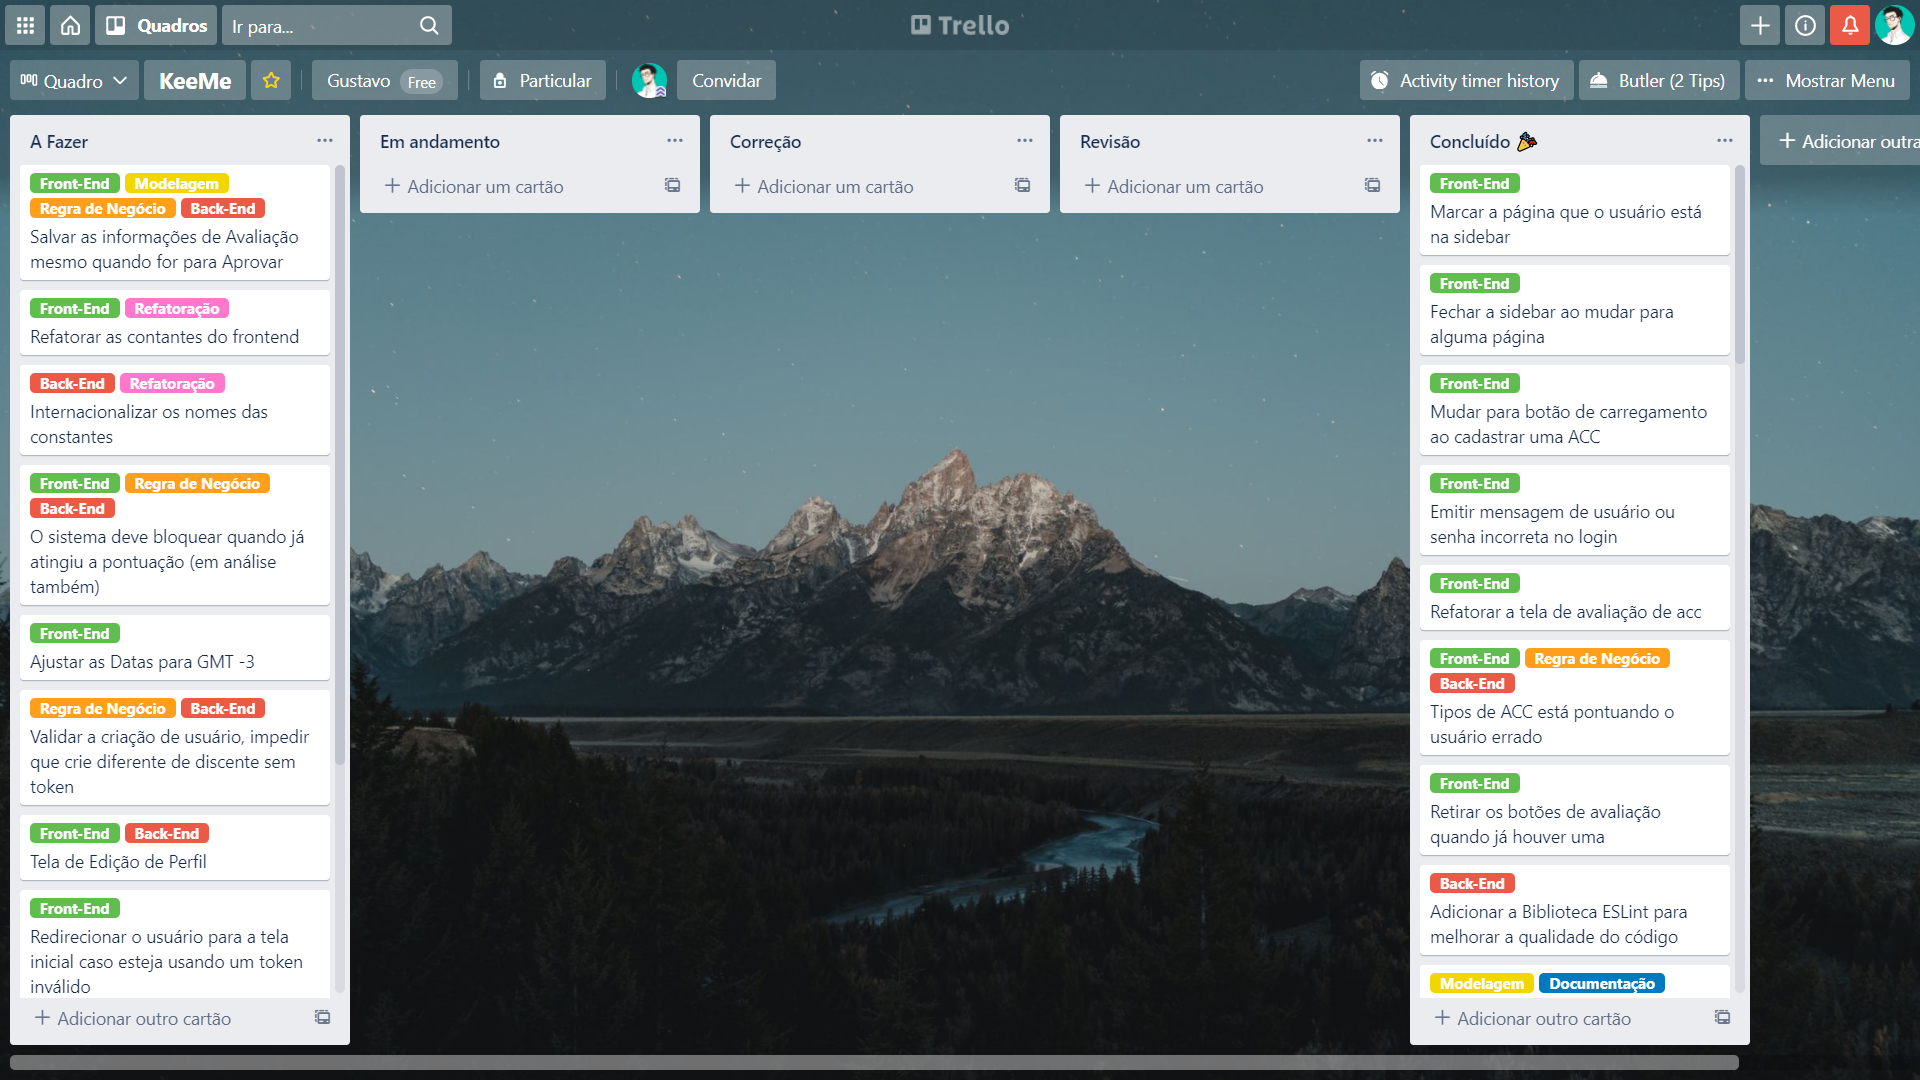
\includegraphics[width=\textwidth]{dados/figuras/Metodologia/trello.png}
    \caption{Quadro no Trello do Projeto KeeMe}
    \label{fig:screenTrelloKeeMe}
\end{figure}

A Figura \ref{fig:screenTrelloKeeMe} mostra o quadro do Trello utilizado no projeto KeeMe. No projeto foram utilizadas 5 colunas, sendo estas: A Fazer, que relaciona todas as tarefas que ainda precisam ser implementadas na aplicação; Em andamento, que é aquilo que está sendo executado no momento; Correção, que reune as tarefas que foram feitas, mas nos quais foram encontradas bugs, ou que não foram desenvolvidas corretamente; A coluna de Revisão, que é aquilo que deve ser testado; E por último a coluna de Concluído, que reúne todas as tarefas que foram executadas, e que foram concluídas da conforme o planejado.

Além da utilização de raias, conforme pode ser visto na \ref{fig:screenTrelloKeeMe}, foram utilizadas também as etiquetas coloridas para melhorar o gerenciamento das tarefas e ter um auxílio visual da área ao qual a tarefa pertence, as etiquetas utilizadas são: \textit{Front-end}, que descreve tudo que deve ser feito da parte visual do sistema; \textit{Back-end}, que é o serviço onde estão as regras de negócio do sistema; Regra de negócio, essa etiqueta se refere a qualquer tarefa que esteja diretamente ligada à regra de negócio, como as pontuações, por exemplo; Modelagem, que diz respeito às tarefas de modelagem dos processos e do banco de dados; Prototipação, que relaciona-se à parte visual do sistema, à tudo que envolva o protótipo do projeto; Documentação, como o nome sugere, é a parte da escrita de documentos relativos ao código, arquitetura, etc, do sistema; Infraestrutura, são tarefas relativas à integração com banco de dados, à hospedagem do site e à forma que os serviços (\textit{Front-end} e \textit{\textit{Back-end}}) da aplicação se comunicam; Refatoração, que é tudo aquilo que foi feito e está funcional, mas que de alguma forma precisa ser melhorado; e por último Banco de Dados, que está diretamente ligado à modelagem e ao \textit{Back-end}, e diz respeito a tudo que envolva o banco de dados da aplicação.

\section{Modelagem}
\label{sec:modelagem}

A modelagem de sistemas serve para que se tenha uma direção clara do que se fazer durante o desenvolvimento da aplicação. A criação de diagramas e modelos serve para que os desenvolvedores saibam exatamente o que deve ser feito, quais as entidades de uma aplicação e como essas entidades relacionam-se entre si, quais os fluxos de funcionalidades, entre outros aspectos inerentes à aplicação sendo desenvolvida. É um fator indispensável na busca pela qualidade na criação de um software.

Para se realizar a modelagem foi utilizada a UML (Unified Modeling Language), segundo \cite{guedes2018uml}, é uma linguagem visual utilizada para modelar softwares baseados no paradigma de orientação a objetos. O UML surge como uma linguagem amplamente utilizada de modelagem, tornando-se o padrão de qualquer equipe de desenvolvimento, e sendo extremamente útil na fase de planejamento de um software. \cite{guedes2018uml} ressalta que a UML não se trata de uma linguagem de programação, além de também não ser um processo de desenvolvimento.

\section{Prototipação}
\label{sec:prototipacao}

A etapa de prototipação do sistema se deu para que fosse possível ser ter uma direção ao qual seguir em relação à interface da aplicação. Dessa forma, assim como se faz necessária a modelagem do banco de dados de uma aplicação de forma a se planejar a interação entre as classes e métodos, também se faz necessária a prototipação da interface da aplicação. Para fazer a modelagem do KeeMe foi utilizada a ferramenta Figma, uma ferramenta de design de interface na qual todo o trabalho é feito através do navegador \cite{interativa2019figma}.

\begin{figure}[H]
    \centering
    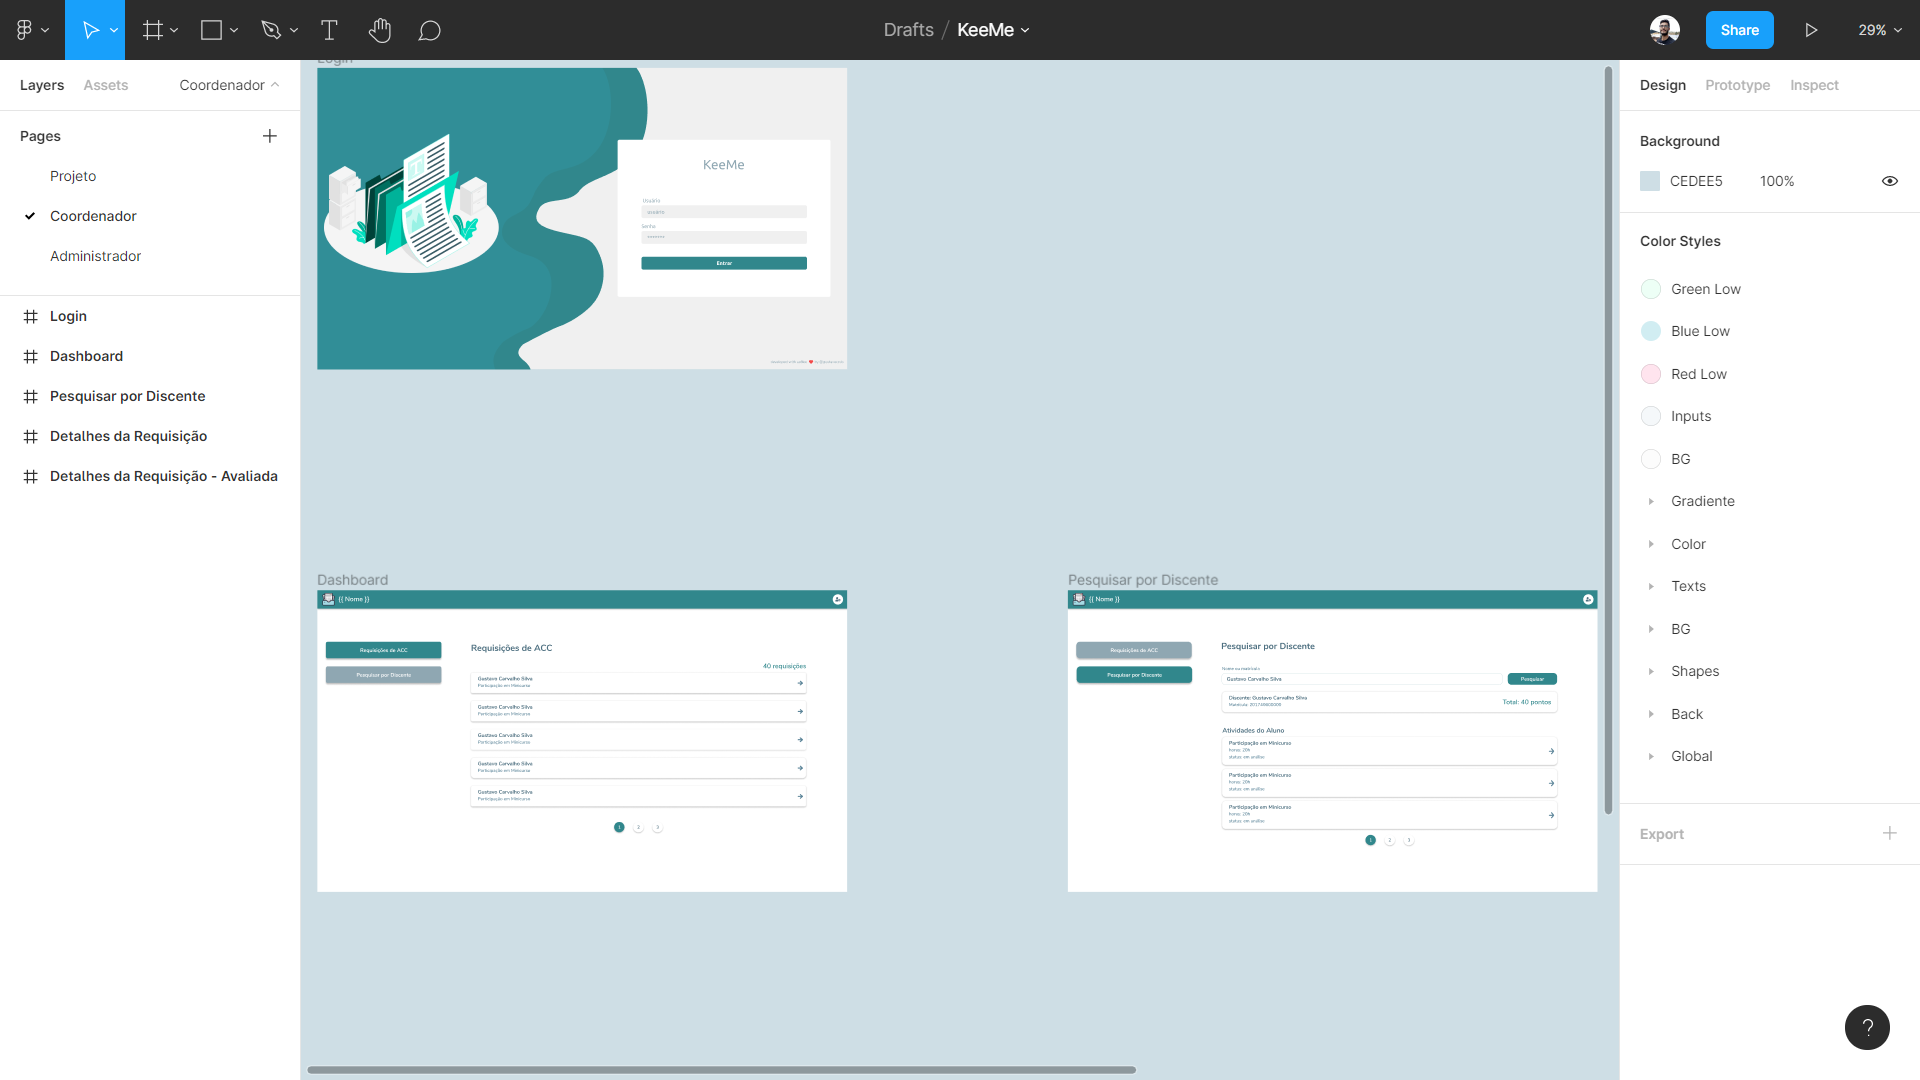
\includegraphics[width=\textwidth]{dados/figuras/Metodologia/figma.png}
    \caption{Prototipo do Projeto KeeMe}
    \label{fig:figmaKeeMe}
\end{figure}

A Figura \ref{fig:figmaKeeMe} mostra um exemplo das telas criadas na prototipação. Neste caso, estão sendo exibidas três telas do módulo do Coordenador, que são as telas de Login, Início e Pesquisa de Discente. 

A utilização de um protótipo permitiu uma melhor visualização da aplicação final, além de servir como um norteador do que deveria ser criado, e do que poderia ser utilizado dentro da aplicação. Após concluído o protótipo\footnote[1]{https://www.figma.com/file/28fcRaEdbWgQkIAw6Pnfwh/KeeMe?node-id=0\%3A1}, foi realizada uma reunião junto à comissão responsável pelo regulamento de ACCs, composta por dois professores e um aluno representante de cada curso da FACEEL. Através dessa reunião a interface, assim como as funcionalidades que ela deveria possuir, foram validadas e aprovadas, permitindo o início da codificação baseada no protótipo.

\section{Tecnologias}
\label{sec:tecnologias}

As tecnologias utilizadas na concepção de um software tem ligação direta com o funcionamento final da aplicação. Dessa forma, a escolha do conjunto de ferramentas deve ser feita com cuidado, considerando o escopo do software desenvolvido.

A modelagem dos diagramas mostrando as relações entre entidades do sistema e dos fluxos de processos foi feita utilizando a aplicação LucidChart descrita por \cite{lucidchart} como sendo uma ferramenta de criação de diagramas inteligentes. Tal escolha se deu pela facilidade na utilização da ferramenta, o que diminuiu a curva de aprendizado, e pelas funcionalidades que a ferramenta apresenta em relação à criação de diagramas.

Tanto o \textit{Back-end} quanto o \textit{Front-end} da aplicação foram construídos utilizando o Node.js como base, como descrito em \cite{node} o Node.js é uma ferramenta que permite a execução de código Javascript, linguagem descrita em \cite{javascript} como uma linguagem linguagem leve, interpretada e baseada em objetos mais conhecida como linguagem de \textit{scripts} para web, sem a necessidade de um navegador. O código do projeto foi escrito em Typescript, que por sua vez é descrito em \cite{typescript} como um superconjunto de Javascript que adiciona novas funcionalidades à linguagem, dentre essas funcionalidades a mais importante é a de tipagem dos dados, algo não existente no Javascript, e que permite um controle melhor das informações que estão sendo manipuladas na aplicação, além da capacidade de criar implementações utilizando programação orientada a objetos no Javascript. Como editor de código, foi escolhido o Visual Studio Code ferramenta desenvolvida pela Microsoft e descrito como um "um editor de código-fonte leve, mas poderoso, que roda em sua área de trabalho e está disponível para Windows, macOS e Linux" \cite{visualstudiocode}.

Como base de dados, foi utilizado o MySQL que segundo \cite{mysql} é um banco de dados que possui bom desempenho, confiabilidade e facilidade de uso, tal escolha se deu pela necessidade da utilização de um banco de dados relacional, que é descrito por \cite{oracle2021bancorelacional} como sendo um tipo de banco de dados que armazena e fornece acesso a pontos de dados relacionados entre si, e que faz a utilização de tabelas e chaves para fazer as relações entre as informações armazenadas. Todas as operações de manipulação de dados do banco e do banco de dados em si são feitas usando a biblioteca TypeORM, descrito em \cite{typeorm} como um ORM (Object-relational mapping, "Mapeamento objeto-relacional") que tem como objetivo trazer suporte às últimas funcionalidades do Javascript, provendo funcionalidades que auxiliam na criação de aplicações que utilizam banco de dados, um ORM é descrito por \cite{fonseca2019orm} como sendo um paradigma de aproximação dos bancos de dados relacionais com a programação orientada a objetos. Para auxiliar na visualização do banco de dados foi utilizado o BeeKeeper Studio, um "gerenciador e editor de SQL de código aberto" \cite{beekeeper}.

O \textit{Front-end} da aplicação foi construído utilizando o React, biblioteca criada por \cite{react} com o foco na construção de interfaces e que permite a manipulação de elementos HTML dentro do Javascript. O React foi escolhido primeiramente pela popularidade da biblioteca, o que impacta na quantidade de documentação e de extensões criadas para a mesma; e pela capacidade de componentização do código, que permite sua reutilização dentro do software, diminuindo o re-trabalho. Em conjunto ao React foi utilizado o \textit{framework} ChakraUI, que de acordo com \cite{chakraui} se trata de uma biblioteca de componentes de interface, a escolha deste \textit{framework} se deu pelo fato de que além de possuir componentes de layout prontos, também permite a personalização desses componentes, facilitando a estilização do software.

Além das tecnologias já citadas, foram utilizados também o Insomnia, que segundo sua documentação em \cite{insomnia} é uma ferramenta de código aberto que permite a chamada de requisições REST, e foi utilizada durante o desenvolvimento para os testes nos serviços providos pelo \textit{Back-end} da aplicação. O REST segundo \cite{costa2020__rest} é um padrão arquitetural de informações trafegadas entre dois diferentes sistemas através de uma rede de internet; A ferramenta Git para o versionamento do código gerado, \cite{git} explica que o Git é uma ferramenta de versionamento de código, que pode ser utilizada desde projetos pequenos, quanto projetos complexos com rapidez e eficiência. O Git permite o rastreamento de alterações no código, comparações com versões anteriores, e permite desfazer alterações que possam ter causado erro no código; Foi utilizado ainda o Lighthouse, uma ferramenta de desenvolvedor de código aberto, que segundo \cite{lighthouse} possui a capacidade de fazer testes automatizados numa página web para avaliar sua qualidade. A ferramenta foi utilizada para avaliar o grau de qualidade da aplicação desenvolvida neste trabalho.
